\chapter{Aplicación sobre datos}

\noindent A lo largo de este capítulo se  aplicarán algunas de las técnicas desarrolladas anteriormente a ejemplos prácticos con bases de datos reales obtenidas de distintos repositorios. 

\noindent La principal herramienta usada ha sido el lenguaje de programación Python, utilizando librerías como Pandas para el manejo de las bases de datos, Scikit-Learn para la implementación de los modelos  y otras librerias de visualización como Matplotlib para la inclusión de gráficos sencillos. 

\section{Tipo de alubias}
\subsection*{Descripción del DataSet}
\noindent Este conjunto de datos,  \cite{Alubias} está formado por 12 variables predictoras que detallan \emph{Koklu, M. y Ozkan, I.A.}\cite{Koklu 2020}. En concreto las medidas son obtenidas mediante imagenes tomadas de distintas variedades de alubias ya clasificadas, en particular, las características medidas son las siguientes:
\begin{enumerate}
\item Área de la alubia medida en pixeles con sus límites incluidos.  
\item Perímetro 
\item Longitud del eje máximo
\item Longitud del eje mínimo
\item Ratio de aspecto, es decir, el cociente entre las dos medidas anteriores. 
\item Excentricidad 
\item Área convexa; número de pixeles en el menor polígono convexo. 
\item Diámetro equivalente
\item 
\item
\item Redondez
\item Compacidad
\end{enumerate}
\subsection*{Objetivos}

\noindent  \emph{Koklu, M. y Ozkan, I.A.}\cite{Koklu 2020} buscan crear distintos predictores que permitan clasificar de manera exitosa los distintos tipos de alubias ya que es complicado certificar la clase de alubia que se tiene. Es por ello que no nos centraremos en ese aspecto predictivo. Para empezar se hará una proyección mediante las variables canónicas 

\subsection*{Métodos a utilizar}
\noindent Para estudiar la estructura de los datos, se utilizará el análisis de componentes principales. Por otro lado, para comprobar la existencia de factores latentes se aplicará el análisis de factores principales. Tras aplicar ambas técnicas,
\subsection*{Desarrollo y resultados}
\subsection*{Conclusiones}

\newpage
\section{Cemento y capacidad predictora}

\subsection*{Descripción del dataset}
\noindent El dataset  \cite{Yeh 2007} es un conjunto de datos recogidos de distintos tipos de cementos con distintas densidades, en particular tenemos las siguientes variables:
\begin{table}[h]
\footnotesize
\centering
\begin{tabular}{|l|l|l|l|}
\hline
Nombre & Tipo de dato & Medida & Descripción \\
\hline
Cemento (variable 1) & continuo & kg en una mezcla m3 & Variable predictora \\
Escoria de alto horno (variable 2) & continuo & kg en una mezcla m3 & Variable predictora \\
Ceniza volante (variable 3) & continuo & kg en una mezcla $m^3$ & Variable predictora \\
Agua (variable 4) & continuo & kg en una mezcla $m^3$ & Variable predictora \\
Superplastificante (variable 5) & continuo & kg en una mezcla $m^3$ & Variable predictora \\
Agregado grueso (variable 6) & continuo & kg en una mezcla $m^3$ & Variable predictora \\
Agregado fino (variable 7) & continuo & kg en una mezcla $m^3$ & Variable predictora \\
Edad & continuo & Día (1-365) & Variable predictora \\
Resistencia a la compresión & continuo & MPa & Variable respuesta \\
\hline
\end{tabular}
\end{table}

\noindent 

\noindent En total se recogen 1030 muestras de las cuales un 70\% se utilizan para el ajuste y un 30\% para construir una estimación del error cuadratico medio de predicción. 
\subsection*{Objetivos} 

\noindent El objetivo es encontrar cual de los modelos utilizados para regresión de los detallados en el trabajo obtiene una mejor capacidad predictiva. 
\subsection*{Desarrollo}
\noindent Se ajustan 3 modelos distintos, un modelo lineal, un árbol de regresión, y una red neuronal. 

\noindent Las características de los modelos y de los procesos de ajuste son los siguientes:

\noindent El modelo lineal es ajustado mediante el método de los minimos cuadrados obteniéndose un mínimo de error cuadrático de $106.14$ en el conjunto de entrenamiento mientras que en el conjunto de testeo se obtiene un error cuadrático medio de $108,215$. Además aunque no se pueda usar en el resto de modelos se obtiene en este caso un coeficiente de determinación $R^2$ de $0,62$ en el conjunto de ajuste. Por tanto, a nivel predictivo el modelo lineal tiene un buen rendimiento. 

\noindent El árbol de decisión utiliza el criterio CART de \emph{Breiman, L.}\cite{Breiman 1984}, ya que es el implementado por defecto en la librería \emph{Scikit-Learn} de Python. Este modelo proporciona un error cuadrático medio de  $108.22$ sobre el conjunto de ajuste mientras que sobre el conjunto de testeo proporciona un error cuadrático de $57.55$, lo que implica que tiene una buena capacidad predictiva. 

\noindent En la red neuronal se ha elegido un modelo simple con dos capas, la primera con 13 neuronas con una función de activación lineal rectificada, en cambio, la otra capa contiene únicamente una neurona con una función lineal. En este caso el ajuste de la red neuronal obtiene un error cuadrático medio de $MSE=40.19$ en el ajuste y un $MSE=41.72$ en el conjunto de prueba, en principio, tenemos un modelo que comete menos error en el conjunto de prueba. 

\noindent Hay que destacar que ninguno de los modelos ha incurrido en problemas de sobreajuste, es decir, no se ha tenido casos en los que el valor del error medio en el conjunto de ajuste sea mucho menor que en el conjunto de prueba. 

\noindent Una vez ajustados los modelos, se pueden tomar los valores predichos para los datos de prueba y graficarlos frente a los valores reales, en cada caso tendremos los puntos en azul y la recta roja representaría los puntos los cuales su predicción es igual al valor real. 

\begin{figure}[ht]
  \centering
  \begin{minipage}{0.32\textwidth}
   
    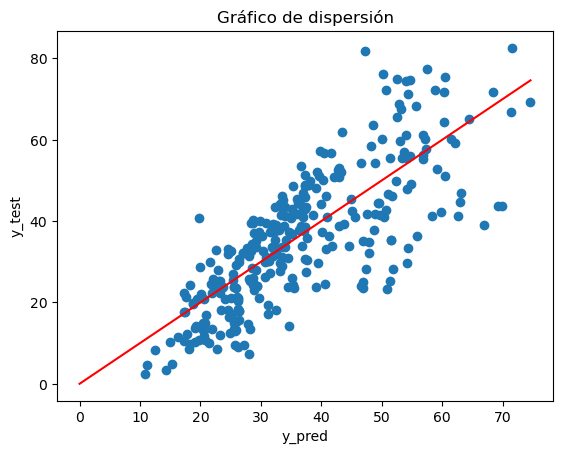
\includegraphics[width=\textwidth]{Documentos Extra/Imagenes/Datos PruebasRegresionLineal.png}
    \caption{Regresión Lineal}
    \label{fig:regresion_lineal}
  \end{minipage}
  \hfill
  \begin{minipage}{0.32\textwidth}
  
    \includegraphics[width=\textwidth]{Documentos Extra/Imagenes/Datos PruebasÁrbolesRegresion.png}
    \caption{Árbol de Regresión}
    \label{fig:regression_tree}
  \end{minipage}
  \begin{minipage}{0.32\textwidth}
    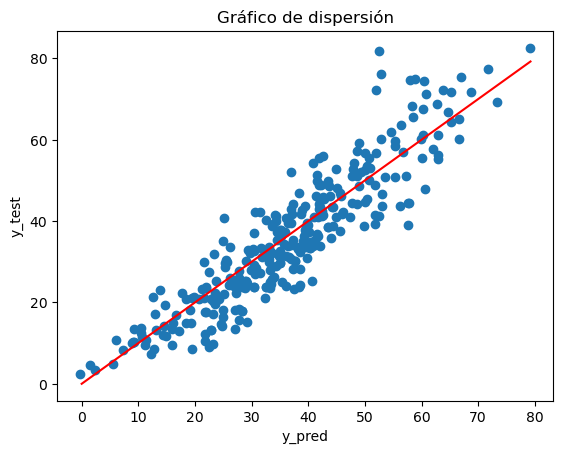
\includegraphics[width=\textwidth]{Documentos Extra/Imagenes/Datos PruebasRedNeuronal.png}
    \caption{Red Neuronal}
    \label{fig:red_neuronal}
  \end{minipage}
 \end{figure}

\noindent Se puede ver que en el caso del modelo lineal \ref{fig:regresion_lineal} los puntos son más lejanos de la recta. 




\subsection*{Conclusiones}
\noindent En resumen, podemos concluir que el modelo lineal no es la mejor opción para realizar predicciones. Aún así este tipo de modelos son útiles para sacar otro tipos de conclusiones como por ejemplo influencias lineales con la variable independiente. 

\noindent En cambio, los modelos de árbol de regresión y la red neuronal proporcionan mejores predicciones de manera altamente significativa con relación a la regresión mediante un modelo lineal.